%!TEX root = ../../super_main.tex

\section{Continuous Integration}
\label{sec:continuous_integration}
As mentioned in \secref{sec:extreme_programming}, we wanted a Continuous Integration (CI) server in order to ensure that our code base always was at a stable state. We installed Jenkins on the same server that makes up the server part of our client-server architecture because it was easily available. Jenkins is an open source automation server, which supports various different plugins that helps with builds, viewing test results, etc. We configured this Jenkins server to be notified whenever our Git version control code repositories (hosted on GitHub) for both Android and PHP code were changed. When this notification happened, Jenkins would build the corresponding project and automatically run its unit tests. Whenever the build projects would go from a previously successful build to a now failing build or vice versa, the Jenkins system would send out mails to our group, so we were aware that something went wrong or that it was now fixed again. If a build failed, the mail would contain information regarding which tests failed, and their stack trace. This made it possible for us to give immediate attention to issues that we did not catch before pushing our content to the version control. \figref{fig:jenkins_front_page} shows the front page of the Jenkins website. In the left side, the build queue can be seen, which shows if any builds are currently running. In the center, the various projects that are currently configured for the Jenkins setup can be seen. The blue circle changes to red if the most recent build was a failure, and besides that, it can be seen how long time has passed since the most recent pass, most recent failure, and how long the last build took to finish. By clicking on one of the projects, statistics can be seen for checkstyes warnings, code coverage, and test results. 

\begin{figure}[!htbp]
    \centering
    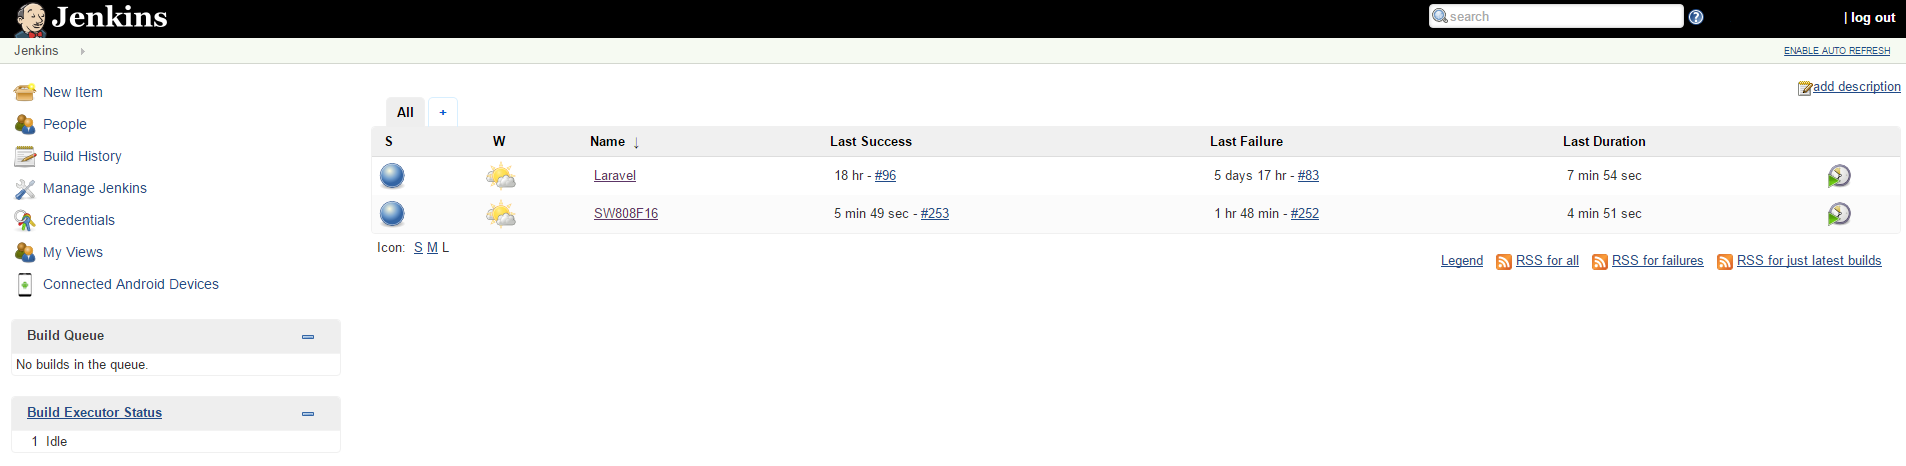
\includegraphics[width=\textwidth]{graphic/quality_assurance/jenkins_frontpage}
    \caption{Jenkins CI front page.}
    \label{fig:jenkins_front_page}
\end{figure}
\FloatBarrier

We used this extensively during the development, because when several people merge their work into the master branch of the version control several times per day, something is bound to go wrong eventually. This ensured that we always knew if something was wrong with either of our projects, so we knew when we needed to allocate people for fixing it. 
